\section{Hausdroff measure}\label{hausdorff_measure}

Let $\omega_s = \pi^{s/2} / \Gamma(1 + s/2)$, $s \geq 0$, $\Gamma$ is Euler gamma function. Note that $\omega_0 = 1$ and if $s = n \in \mathbb{N}$, then $\omega_n$ is the volume of the unit ball in $\mathbb{R}^n$.\footnote{See Appendix \ref{appendix_b}.}And the volume of ball $B = B^n(x,r) \subset \mathbb{R}^n$ equals 
\begin{align*}
    \operatorname{vol}(B) = \omega_n r^n = \frac{\omega_n}{2^n} \left(\operatorname{diam} B\right)^n.
\end{align*}

Let $X$ be a metric space, $d \geq 0$. For any $\varepsilon > 0$ and any $E \subset X$, we define
\begin{align*}
    \mathcal{H}^s_{\varepsilon}(E) = \inf \frac{\omega_s}{2^s} \sum^\infty_{i=1} \left(\operatorname{diam} A_i\right)^s,
\end{align*}
where the infimum is taken over all possible coverings
\begin{align*}
    E \subset \bigcup^\infty_{i=1} A_i, \,\, \text{with} \,\, \operatorname{diam} A_i < \varepsilon.
\end{align*}
Sometimes, $\H^s_\varepsilon(E)$ is called $\varepsilon$-{\em approximate} $s$-{\em dimensional Hausdorff measure} of $E$\cite{5}.

Note that the function $\varepsilon \mapsto \mathcal{H}^s_{\varepsilon}$ is nonincreasing. Indeed, if $\varepsilon_1 > \varepsilon_2$, then there are more $A_i$ in family $\{A_i\}$ with $\operatorname{diam} A_i < \varepsilon_1$ than that with $\operatorname{diam} A_i < \varepsilon_2$. Then $\mathcal{H}^s_{\varepsilon_1}(E)$ is the infimum over a bigger set of coverings than $\mathcal{H}^s_{\varepsilon_2}(E)$ and hence 
\begin{align*}
    \mathcal{H}^s_{\varepsilon_1}(E) \leq \mathcal{H}^s_{\varepsilon_2}(E).
\end{align*}
Since $\varepsilon \mapsto \mathcal{H}^s_{\varepsilon}$ is nonincreasing, then the limit
\begin{align*}
    \mathcal{H}^s(E) = \lim_{\varepsilon \to 0} \mathcal{H}^s_{\varepsilon}(E)
\end{align*}
exists and is called Hausdroff $h$-measure of $E$.\footnote{Hausdorff $h$-measure and Hausdorff $h$-content are from \cite{6} \label{footnote_hausdorff_content}.}Also, $\mathcal{H}^s(E)$ can be defined as
\begin{align*}
    \mathcal{H}^s(E) = \sup_{\varepsilon > 0} \H^s_\varepsilon(E).
\end{align*}

\medskip

\begin{definition}
$\mathcal{H}^s(E)$ is called ($s$-dimensional) Hausdorff measure and $\mathcal{H}^s: P(X) \to [0,\infty]$.
\end{definition}

\medskip

\begin{remark}
For any $\varepsilon > 0$, $\mathcal{H}^s_{\varepsilon}(E) \leq \mathcal{H}^s(E)$ and if $s = 0$, $\mathcal{H}^0$ is the counting measure. In particular, Hausdorff $h$-content of $E$ is defined as:\textsuperscript{{\rm \ref{footnote_hausdorff_content}}}
\begin{align*}
    \mathcal{H}^n_{\infty}(E) = \inf \frac{\omega_s}{2^s} \sum^\infty_{i=1} \left(\operatorname{diam} A_i\right)^s,
\end{align*}
where the infimum is taken over all possible coverings
\begin{align*}
    E \subset \bigcup^\infty_{i=1} A_i.
\end{align*}
Also, it is easy to see that $\mathcal{H}^s(E) = 0$ if and only if $\mathcal{H}_\infty^s(E) = 0$, and we will prove it.
\end{remark}

\medskip

\begin{proposition}
If $0 < s < \infty$ and $E \subset X$ is a subset of a metric space, then $\mathcal{H}^s(E) = 0$ if and only if $\mathcal{H}_\infty^s(E) = 0$.
\end{proposition}
\begin{proof}
~\begin{enumerate}
    \item[($\Rightarrow$)] If $\H^s(E) = 0$, then  $\H^s_\infty(E) = 0$ follows easily. Indeed, \begin{align*}
        \H^s_\infty(E) \leq \inf \frac{\omega_s}{2^s} \sum_{i=1}^\infty (\operatorname{diam} A_i)^s = \H^s_\varepsilon(E) \xrightarrow[]{\varepsilon \to 0} \H^s(E),
    \end{align*}  
    since the infimum is taken over all coverings $E \subset \bigcup^\infty_{i=1} A_i$ with $\operatorname{diam} A_i < \varepsilon$, which is a smaller collection of coverings.
    
    \item[($\Leftarrow$)] If $\H^s_\infty(E) = 0$, then for any $\varepsilon > 0$, there exists a covering $\{G^\varepsilon_i\}$ of $E$ with $\operatorname{diam} G^\varepsilon_i < \varepsilon^{1/s}, i = 1,2,\cdots$. Otherwise, there exists $\varepsilon > 0$ such that for all coverings $\{G_i\}$ of $E$ with $\operatorname{diam} G_i \geq \varepsilon^{1/s}$, $\H^s_\infty(E) = 0$, which is a contradiction.\footnote{This proof is in: \url{https://www.math.stonybrook.edu/~rdhough/mat639-spring17/lectures/lecture20.pdf}.}Letting $\varepsilon \to 0$ implies
    \begin{align*}
        \H^s(E) = \lim_{\varepsilon^{1/s} \to 0}\H^s_{\varepsilon^{1/s}}(E) \leq \lim_{\varepsilon^{1/s} \to 0} \frac{\omega_s}{2^s} \sum^\infty_{i=1} (\operatorname{diam} G^\varepsilon_i)^s = 0, \quad \operatorname{diam} G^\varepsilon_i < \varepsilon^{1/s}.
    \end{align*}
\end{enumerate}
\end{proof}


\medskip

\begin{example}
Let $X = \mathbb{R}^n$, $B = B^n(x,r)$, then $\mathcal{H}^n_{\infty}(B) \leq \operatorname{vol}(B)$. Indeed,
\begin{align*}
    \mathcal{H}^n_{\infty}(B) = \inf \frac{\omega_n}{2^n} \sum^\infty_{i=1} \left(\operatorname{diam} A_i\right)^n \leq \frac{\omega_n}{2^n} \sum^\infty_{i=1} \left(\operatorname{diam} A_i\right)^n = \operatorname{vol}(B).
\end{align*}
\end{example}

\medskip

\begin{theorem}
For any $0 < \varepsilon \leq \infty$, $\operatorname{vol}(B) = \mathcal{H}^n_{\varepsilon}(B) = \mathcal{H}^s(B)$.
\end{theorem}

\medskip

We will prove this theorem later.

\medskip

\begin{theorem}
$\mathcal{H}^s$ is a metric outer measure.
\end{theorem}
\begin{proof}
~\begin{enumerate}[label=(\alph*)]
    \item In order to prove $\mathcal{H}^s: P(X) \to [0,\infty]$ is an outer measure, it suffice to show that
    \begin{enumerate}[label=\arabic*)]
        \item $\mathcal{H}^s(\emptyset) = 0$, and this is obvious.
    
        \item If $A \subset B$, then $\mathcal{H}^s(A) \leq \mathcal{H}^s(B)$, and this is also obvious.
    
        \item For all $E_1, E_2, \cdots \in X$, 
        \begin{align*}
            \mathcal{H}^s\left(\bigcup^\infty_{n=1} E_n\right) \leq \sum^\infty_{n=1} \mathcal{H}^s(E_n).
        \end{align*}
    
        Assume that the right hand side is finite. Then, for any $\varepsilon > 0$, by $\mathcal{H}^s_\varepsilon \leq \mathcal{H}^s$, we have
        \begin{align*}
            \sum^\infty_{n=1} \mathcal{H}^s_\varepsilon(E_n) < \infty.
        \end{align*}
        For fixed $\delta > 0$, there exists a covering for each $E_n$,
        \begin{align*}
            E_n \subset \bigcup^\infty_{i=1} A_{ni},\quad  \operatorname{diam} A_{ni} < \varepsilon,
        \end{align*}
        such that
        \begin{align*}
            \mathcal{H}^s_\varepsilon(E_n) \geq \frac{\omega_s}{2^s} \sum^\infty_{i=1} \left(\operatorname{diam} A_{ni}\right)^s - \frac{\delta}{2^n}.
        \end{align*}
        Then,
        \begin{align*}
            \sum^\infty_{n=1} \mathcal{H}^s_\varepsilon(E_n) \geq \frac{\omega_s}{2^s} \sum^\infty_{n,i=1} \left(\operatorname{diam} A_{ni}\right)^s - \delta \geq \mathcal{H}^s_\varepsilon \left(\bigcup^\infty_{n=1} E_n\right) - \delta,
        \end{align*}
        where the last step comes from $\bigcup^\infty_{n=1} E_n \subset \bigcup^\infty_{n,i=1} A_{ni}, \operatorname{diam} A_{ni} < \varepsilon$ and the definition of $\mathcal{H}^s_\varepsilon$. Letting $\delta \to 0$ yields
        \begin{align*}
            \sum^\infty_{n=1} \mathcal{H}^s(E_n) \geq \sum^\infty_{n=1} \mathcal{H}^s_\varepsilon (E_n) \geq \mathcal{H}^s_\varepsilon \left(\bigcup^\infty_{n=1} E_n\right).
        \end{align*}
        Also, letting $\varepsilon \to 0$ 
        \begin{align*}
            \sum^\infty_{n=1} \mathcal{H}^s(E_n) \geq \mathcal{H}^s \left(\bigcup^\infty_{n=1} E_n\right).
        \end{align*}
    \end{enumerate}
    
    \item 
    It remains to show that $\mathcal{H}^s$ is a metric outer measure, that is, for any $E, F \subset X$ and $\operatorname{dist}(E,F) > 0$, \begin{align*}
        \mathcal{H}^s(E \cup F) = \mathcal{H}^s(E) + \mathcal{H}^s(F).
    \end{align*}
    And it suffices to show that for any $\varepsilon < \operatorname{dist}(E,F)$,
    \begin{align*}
        \mathcal{H}^s_\varepsilon(E \cup F) = \mathcal{H}^s_\varepsilon(E) + \mathcal{H}^s_\varepsilon(F).
    \end{align*}
    
    \begin{enumerate}[label=\arabic*)]
        \item Let $\{A_i\}$ be a covering for $E \cup F$, such that
        \begin{align*}
            E \cup F \subset \bigcup^\infty_{i=1} A_i, \,\, \text{with} \,\, \operatorname{diam} A_i < \varepsilon,
        \end{align*}
        and assume that $A_i \cap (E \cup F) \neq \emptyset$ for all $i \in \mathbb{N}$, since otherwise we could remove this $A_i$ from the covering. Since $\operatorname{diam} A_i < \varepsilon < \operatorname{dist}(E,F)$, then each $A_i$ has a nonempty intersection with only one set $E$ or $F$. Then the family $\{A_i\}_i$ can be split into two disjoint subfamilies
        \begin{align*}
            \{B_j\}_j & = \{A_j\, |\, A_j \cap E \neq \emptyset\}, \\
            \{C_j\}_j & = \{A_j\, |\, A_j \cap F \neq \emptyset\},
        \end{align*}
        and $E \subset \bigcup^\infty_{j=1} B_j$, $F \subset \bigcup^\infty_{j=1} C_j$. Hence,
        \begin{align*}
            \frac{\omega_s}{2^s} \sum^\infty_{i=1} \left(\operatorname{diam} A_i\right)^s & = \frac{\omega_s}{2^s} \sum^\infty_{j=1} \left(\operatorname{diam} B_i\right)^s + \frac{\omega_s}{2^s} \sum^\infty_{j=1} \left(\operatorname{diam} C_i\right)^s \\
            & \geq \mathcal{H}^s_\varepsilon(E) + \mathcal{H}^s_\varepsilon(E).
        \end{align*}
        Since $\{A_i\}_i$ is an arbitrary covering of $E \cup F$, then taking infimum over coverings yields
        \begin{align*}
            \mathcal{H}^s_\varepsilon(E \cup F) \geq \mathcal{H}^s_\varepsilon(E) + \mathcal{H}^s_\varepsilon(E).
        \end{align*}
        
        \item The opposite inequality is obvious. Suppose $\{B_j\}_j$ and $\{C_j\}_j$ are coverings for $E$ and $F$ respectively, with $\operatorname{diam}(B_j) < \varepsilon$ and $\operatorname{diam}(C_j) < \varepsilon$. Let $C_i$ be replaced by $D_i = C_i \cap F$ and $B_i$ remain the same. Then, $\operatorname{diam}(D_i) \leq \operatorname{diam}(C_i) < \varepsilon$.
        
        Now we can arrange $B_j$ and $D_j$ into a new family $\{A_i\}_i = \{B_i, D_i\}_i$, which is a covering of $E \cup F$. Hence,
        \begin{align*}
            \frac{\omega_s}{2^s} \sum^\infty_{j=1} \left(\operatorname{diam} B_j\right)^s + \frac{\omega_s}{2^s} \sum^\infty_{j=1} \left(\operatorname{diam} C_j\right)^s & \geq \frac{\omega_s}{2^s} \sum^\infty_{i=1} \left(\operatorname{diam} A_i\right)^s \geq \mathcal{H}^s_\varepsilon(E \cup F),
        \end{align*}
        then taking infimum over coverings yields
        \begin{align*}
            \mathcal{H}^s_\varepsilon(E) + \mathcal{H}^s_\varepsilon(E) \geq \mathcal{H}^s_\varepsilon(E \cup F).
        \end{align*}
    \end{enumerate}
\end{enumerate}
Thus, $\mathcal{H}^s$ is a metric outer measure.
\end{proof}

\medskip

\begin{corollary}\label{coro_14}
$\mathcal{H}^s$ is countable additive measure on the class of all Borel sets $\mathfrak{B}(X)$.
\end{corollary}

\medskip

\begin{exercise}\label{exercise_12}
Prove that
\begin{enumerate}[label=(\alph*)]
    \item if $\mathcal{H}^s(E) < \infty$, then $\mathcal{H}^t(E) = 0$ for all $t > s$;
    
    \item if $\mathcal{H}^s(E) > 0$, then $\mathcal{H}^t(E) = \infty$ for all $0 < t < s$.
\end{enumerate}
\end{exercise}
\begin{proof}
~\begin{enumerate}[label=(\alph*)]
    \item Since $\H^s(E) < \infty$, then for each $\varepsilon > 0$, there exists family $\{A_i\}$ of open sets $A_i$ with $\operatorname{diam} A_i < \varepsilon$, such that $E \subset \bigcup^\infty_{i=1} A_i$ and
    \begin{align*}
        \frac{\omega_s}{2^s} \sum^\infty_{i=1} (\operatorname{diam} A_i)^s \leq \H^s(E) + 1.
    \end{align*}
    Thus, we have
    \begin{align*}
        \H^t_{\varepsilon}(E) & \leq \frac{\omega_t}{2^t} \sum^\infty_{i=1} (\operatorname{diam} A_i)^s (\operatorname{diam} A_i)^{t - s} \leq \frac{\omega_t}{2^t} \sum^\infty_{i=1} \varepsilon^{t - s} (\operatorname{diam} A_i)^s \\
        & \leq \frac{\omega_t}{2^t} \frac{2^s}{\omega_s} \varepsilon^{t-s} \left( \H^s(E) + 1\right) \xrightarrow[]{\varepsilon \to 0} 0.
    \end{align*}
    
    \item It follows the similar argument in (a).\footnote{This proof is based on: \url{https://www.math.cuhk.edu.hk/course_builder/1415/math5011/MATH5011_Chapter_3.2014.pdf}, with a different definition of $\mathcal{H}^s_{\varepsilon}$.}Another way to prove this is interchanging the positions of $s$ and $t$ in the contrapositive of (b),\footnote{Interchanging $s$ and $t$ is based on the proof in: \url{https://www.math.uchicago.edu/~may/VIGRE/VIGRE2009/REUPapers/Shah.pdf}.} which is 
    \begin{align*}
        \exists t \in (0,s), \H^t(E) < \infty \Longrightarrow \H^s(E) = 0,
    \end{align*}
    and it gives (a), and hence it proves (b).
\end{enumerate}
\end{proof}

\medskip

\begin{remark}
This exercise implies that at most one $s \geq 0$ such that $\mathcal{H}^s(E) < \infty$.
\end{remark}

\medskip

\begin{definition}
The Hausdorff dimension is defined as follows. If $\mathcal{H}^s(E) > 0$ for all $s \geq 0$, then $\dim_{\mathcal{H}}(E) = \infty$ (in this case, $\mathcal{H}^s(E) = \infty$ for all $s \geq 0$). Otherwise, we define
\begin{align*}
    \dim_{\mathcal{H}}(E) = \inf \{s \geq 0\, |\, \mathcal{H}^s(E) = 0 \}.
\end{align*}
\end{definition}

It follows from the Exercise \ref{exercise_12} that there is $s \in [0,\infty]$ such that $\mathcal{H}^t(E) = 0$ for $t > s$ and $\mathcal{H}^t(E) = \infty$ for $0 < t < s$. Then, the Hausdorff dimension of $E$ equals $s$.

\medskip

\begin{example}[The Cantor set]
The Cantor set is constructed as follows:
\begin{enumerate}[label=(\alph*)]
    \item Let $\CC_1$ be the interval $[0,1]$.
    \item Remove the segment $\left(1/3,2/3\right)$, and let $\CC_2$ be the union of the interval of $\left[0,1/3\right],\left[1/3,1\right]$.
    \item Remove the middle thirds of these two intervals and let $\CC_3$ be the union of $\left[0,1/9\right]$, $\left[2/9,1/3\right]$, $\left[6/9,7/9\right]$ and $\left[8/9,1\right]$.
    \item Continue this way and we can get a sequence of compact sets $\CC_n$, such that $\CC_1\supset \CC_2\supset \CC_3\supset\cdots$ and $\CC_n$ is the union of $2^n$ intervals with length $3^{-n}$.
\end{enumerate}
Then the Cantor set is defined as $$\CC = \bigcap^\infty_{i=1}\CC_i.$$ and shown as below:\footnote{Figure source: \url{https://en.wikipedia.org/wiki/File:Cantor_set_in_seven_iterations.svg}.}
\begin{figure}[H]
    \centering
    \includegraphics[width=0.9\textwidth]{Cantor_set_in_seven_iterations}
    \caption{Cantor set in seven iterations.}
    \label{fig:Cantor_set}
\end{figure}
One can prove that the Cantor set is uncountable. 
\end{example}

\medskip

\begin{theorem}
Cantor set is uncountable.
\end{theorem}
\begin{proof}\footnote{This proof is by Gerald Edgar: \url{https://math.stackexchange.com/a/250762}.}Instead of the diagonal proof directly, we use Cantor's first proof of uncountability. Let $C$ be the cantor set, and let $E = \{u_1,u_2,\cdots\}$ be a countable set. We construct a point of $\CC$ but not in $E$. First, $\CC \subseteq [0,1/3] \cup [2/3,1]$, and point $u_1$ does not belong to both of those intervals, so there is an interval $I_1$of length $1/3$ (one of the ones in the first stage of the construction of the Cantor set) with $u_1 \notin I_1$. Now when we remove the middle third of $I_1$ we get two intervals of length $1/3^2$. As before, $u_2$ does not belong to both of these intervals, so there is an interval $I_2 \subset I_1$ of length $1/3^2$ (one of the ones in the second stage of the construction of the Cantor set) with $u_2 \notin I_2$. Continue in this way to get $I_1 \supset I_2 \supset I_3 \supset \cdots \supset I_k \supset \cdots$ where $I_k$ has length $1/3^k$ (one of the intervals in the kth stage of the construction of the Cantor set) and $u_k \notin I_k$. Finally, we get a point $x \in \bigcap^\infty_{k=1} I_k$ where $x \in \CC$ but $x \neq u_k$ for all $k$.
\end{proof}

\medskip

Next, we show a result regarding to the Hausdorff  dimension of the Cantor set.

\medskip

\begin{exercise}\label{exe_13}
Let $\CC \subset [0,1]$ be the ternary Cantor set. Prove that $\dim_{\H}(\CC) \leq \log 2/\log 3$.
\end{exercise}
\begin{proof}
Cantor set $\CC$ can be covered by $1$ segment of length $1$, or $2$ segments of length $1/3$, or $4$ segments of length $1/3^2$, $\cdots$, or $2^n$ segments of length $3^{-n}$ and so on. Let $s = \log 2/\log 3$, then by the definition of $\H^s_{\varepsilon}$, we have
\begin{align*}
    \H^s_{3^{-n}}(\CC) \leq \frac{\omega_s}{2^s} 2^n \left(3^{-n}\right)^s.
\end{align*}
Note that $3^s = \left(e^{\log 3}\right)^{\log 2/\log 3} = 2$ and $\left(3^{-n}\right)^3 = 2^{-n}$, then 
\begin{align*}
    \H^s_{3^{-n}}(\CC) \leq \frac{\omega_s}{2^s} 2^n \left(3^{-n}\right)^s = \frac{\omega_s}{2^s},
\end{align*}
letting $n \to \infty$ implies $\H^s(\CC) \leq \omega_s / 2^s$. Thus, $\dim_{\H}(\CC) \leq \log 2/\log 3$.
\end{proof}

\medskip

Furthermore, $\dim_{\H}(\CC) = \log 2/\log 3$. It follows from the following theorem.

\medskip

\begin{theorem}\footnote{See Appendix \ref{appendix_c} for the proof of this theorem.}
For the Cantor set $\CC$, then
\begin{align*}
    \H^s(\CC) = \frac{\omega_s}{2^s}, \quad s = \frac{\log 2}{\log 3}.
\end{align*}
\end{theorem}

\medskip

\begin{example}[Koch snowflak]
Let's introduce von Koch snowflake $K$ show as below:\footnote{Figure source: \url{https://en.wikipedia.org/wiki/File:KochFlake.svg}.}
\begin{figure}[H]
    \centering
    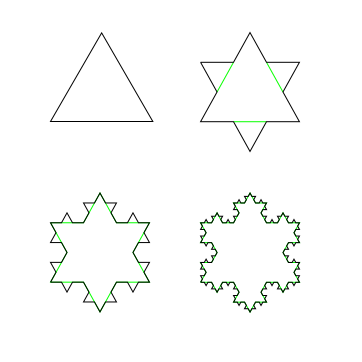
\includegraphics[width=0.3\textwidth]{KochFlake}
    \caption{The first four iterations of the Koch snowflake.}
    \label{fig:koch_snowflake}
\end{figure}

Then $K$ is homeomorphic to the circle $S^1$. For $s = \log/\log 3$, then we have $0 < \H^s(K) < \infty$ and in fact,
\begin{align*}
    \dim_{\H}(K) = \frac{\log 4}{\log 3}.
\end{align*}
\end{example}

\medskip

\begin{proposition}\label{prop_15}
In the definition of the Hausdorff measure, we can always assume that
\begin{enumerate}[label=(\alph*)]
    \item all sets $A_i$ are closed;
    
    \item or all sets $A_i$ are open.
\end{enumerate}
\end{proposition}
\begin{proof}
~\begin{enumerate}[label=(\alph*)]
    \item It is obvious, since $\operatorname{diam} \overline{A_i} = \operatorname{diam} A_i$ and we can replace $A_i$ by its closure.
    
    \item For any $E$ and fixed $\delta > 0$, there exists a family $\{A_i\}$ such that
    \begin{align*}
        \frac{\omega_s}{2^s} \sum^\infty_{i=1} (\operatorname{diam} A_i)^s \leq \H^s_{\varepsilon}(E) + \frac{\delta}{2}, \quad \operatorname{diam} A_i < \varepsilon.
    \end{align*}
    Let $U_i = \bigcup_{x \in A_i} B(x, r_i)$ such that $A_i \subset U_i$, and $U_i$ is open. Also, 
    \begin{align*}
        \operatorname{diam} U_i \leq \operatorname{diam} A_i + 2r_i < \varepsilon,
    \end{align*}
    for some $r_i$ small enough. And we can take $r_i$ small such that
    \begin{align*}
        \frac{\omega_s}{2^s} (\operatorname{diam} U_i)^s \leq \frac{\omega_s}{2^s} (\operatorname{diam} A_i)^s + \frac{\delta}{2^{i+1}}.
    \end{align*}
    
    Then, since $\{U_i\}$ is also a covering of $E$ with $\operatorname{diam} U_i < \varepsilon$, then
    \begin{align*}
        \H^s_{\varepsilon}(E) \leq \frac{\omega_s}{2^s} (\operatorname{diam} U_i)^s \leq \frac{\omega_s}{2^s} (\operatorname{diam} A_i)^s + \frac{\delta}{2} \leq \H^s_{\varepsilon}(E) + \delta,
    \end{align*}
    which implies
    \begin{align*}
        \H^s_{\varepsilon}(E) = \inf \frac{\omega_s}{2^s} (\operatorname{diam} U_i)^s,
    \end{align*}
    and the infimum is taken over all open coverings $\{U_i\}$.
\end{enumerate}
\end{proof}

\medskip

\begin{corollary}\label{coro_15}
In the definition of $\H^s$ on $\mathbb{R}$, we can take coverings by open intervals.
\end{corollary}
\begin{proof}
We can take coverings by open sets, but each open set is contained in an open interval of equal diameter.
\end{proof}

\medskip

Recall that $\H^s$ is a metric outer measure on a metric space $X$. Also, $\H^s$ restricted to $\BB(X)$ is countably additive, i.e. $\H^s$ is a Borel measure.\footnote{A {\em Borel measure} is any measure $\mu$  defined on the $\sigma$-algebra of Borel sets\cite{4}.}

\medskip

\begin{theorem}\label{theorem_119}
$\H^1$ is a measure on $\BB(\mathbb{R})$ such that
\begin{align}\label{theorem_119_1}
    \H^1((a,b)) = b - a,
\end{align}
if $- \infty < a < b < \infty$. Moreover, $\H^1$ is a unique measure with this property, that is, if $\mu$ is a measure on $\BB(\mathbb{R})$ such that $\mu((a,b)) = b - a$ if $- \infty < a < b < \infty$, then $\mu(E) = \H^1(E)$ for all $E \in \BB(\mathbb{R})$.
\end{theorem}

\medskip

$\H^1$ is a measure on $\BB(\mathbb{R})$. Assuming condition (\ref{theorem_119_1}), the uniqueness is easy to prove. 

\medskip

\begin{theorem}\label{theorem_120}
Let $X$ be a metric space, $\mu$ is a measure on $\BB(X)$, $X = \bigcup^\infty_{i=1}U_i$, where $U_i$ is open and $\mu(U_i) < \infty$. Suppose $\nu$ is another measure such that for any open set $U \subset X$, $\nu(U) = \mu(U)$, then for any $E \in \BB(X)$, $\nu(E) = \mu(E)$.
\end{theorem}
\begin{proof}
Since $X$ is a countable union of open sets with finite measure, by Theorem \ref{theorem_114}, then
\begin{align*}
    \mu(E) = \inf_{\substack{U \subset E\\ U - \text{open}}} \mu(U) = \inf_{\substack{U \subset E\\ U - \text{open}}} \nu(U) = \nu(E).
\end{align*}
\end{proof}

\medskip

Now let's use this theorem to prove the uniqueness of the previous theorem.

\medskip

\begin{proof}[Proof of Theorem \ref{theorem_119}]
~\begin{enumerate}[label=(\alph*)]
    \item Since $\H^1((a,b)) = \mu((a,b))$, by Corollary \ref{coro_15}, $\H^1(U) = \mu(U)$ for any open set $U \subset \mathbb{R}$. Thus, by Theorem \ref{theorem_120}, $\H^1(E) = \mu(E)$ for any $E \in \BB(\mathbb{R})$. Hence, the uniqueness is proved.
    
    \item It remains to prove that $\H^1((a,b)) = b - a$. 

    First, for any $\varepsilon > 0$, divide $[a,b]$ into small intervals $I_1, I_2, \cdots$, such that $\operatorname{diam} I_i < \varepsilon$. Note that $\sum^\infty_{i=1}\operatorname{diam} I_i = b - a$. Then,
    \begin{align*}
        \H^1_{\varepsilon}([a,b]) \leq \frac{\omega_1}{2^1} \sum^\infty_{i=1}(\operatorname{diam} I_i)^1 = b - a,
    \end{align*}
    since $\omega_1 = \operatorname{vol}\left(B^1(0,1)\right) = \operatorname{vol}\left((-1,1)\right) = 2$. Letting $\varepsilon \to 0$ gives $\H^1([a,b]) \leq b - a$.
    
    Second, taking infimum over coverings by open intervals $[a,b] \subset \bigcup^\infty_{i=1}U_i$, where $U_i$ is open interval and $\operatorname{diam} U_i < \varepsilon$ and then we have
    \begin{align*}
        \H^1_{\varepsilon}([a,b]) = \inf \sum^\infty_{i=1} \operatorname{diam} U_i.
    \end{align*}
    Since $[a,b]$ is compact, then there exists finite coverings of $[a,b]$ by open intervals. Choose a finite open covering $\{I_i\}$ from $\{U_i\}$ such that $[a,b] \subset \bigcup^k_{i=1} I_i$, then 
    \begin{align*}
        \sum^\infty_{i=1}\operatorname{diam} U_i \geq \sum^k_{i=1} \operatorname{diam}I_i \geq b - a.
    \end{align*}
    Taking infimum over all covering by open intervals with $\operatorname{diam}U_i < \varepsilon$ implies
    \begin{align*}
        \H^1([a,b]) = \inf \sum^\infty_{i=1} \operatorname{diam}U_i \geq b - a.
    \end{align*}
    
    It follows that $\H^1([a,b]) = b - a$, and thus $\H^1((a,b)) = b - a$.
\end{enumerate}
\end{proof}

\medskip

Let's talk more about properties of the Hausdorff measure.

\medskip

\begin{theorem}\label{theorem_121}
For $0 \leq s < \infty$ and every $E \subset X$ (not necessarily measurable), there is a sequence of open sets $V_1 \supset V_2 \supset V_3 \supset \cdots \supset E$ such that 
\begin{align*}
    E \subset \widetilde{E} \coloneqq \bigcap^\infty_{i=1} V_i,
\end{align*}
and $\H^s(E) = \H^s (\widetilde{E})$.
\end{theorem}
\begin{proof}
Note that $\widetilde{E}$ is $G_\delta$ set and hence Borel.

If $\H^s(E) = \infty$, take $v_i = X$ for all $I \in \mathbb{N}$ would yield the statement.

If $\H^s(E) < \infty$, by Proposition \ref{prop_15}, we can taking coverings by open sets in the definition of $\H^s$. So, we could find a covering $\{U_{i_j}\}$ such that
\begin{align*}
    E \subset \bigcup^\infty_{j=1} U_{i_j} \coloneqq U_i, \quad \operatorname{diam} U_{i_j} < \frac{1}{i}.
\end{align*}
and by the definition of $\H^s_{1/i} (E)$, we have
\begin{align*}
    \frac{\omega_s}{2^s} \sum^\infty_{j=1} \left(\operatorname{diam} U_{i_j}\right)^s \leq \H^s_{1/i} (E) + \frac{1}{i}.
\end{align*}

Let $V_i = \bigcap^i_{k=1}U_k$ be open, and clearly, $V_1 \supset V_2 \supset V_3 \supset \cdots \supset E$. Also, 
\begin{align*}
    \widetilde{E} \coloneqq \bigcap^\infty_{i=1} V_i = \bigcap^\infty_{i=1} U_i.
\end{align*}

We need to prove that $\H^s(E) = \H^s (\widetilde{E})$, and since $E \subset \widetilde{E}$ implies $\H^s(E) \leq \H^s(\widetilde{E})$, it remains to prove that $\H^s(E) \geq \H^s(\widetilde{E})$. Clearly,
\begin{align*}
    \widetilde{E} \subset U_i = \bigcup^\infty_{j=1} U_{i_j},
\end{align*}
then $\{U_{i_j}\}$ is a covering of $\widetilde{E}$ with $\operatorname{diam} U_{i_j} < 1/i$. Therefore,
\begin{align*}
    \H^s_{1/i}(\widetilde{E}) \leq \frac{\omega_s}{2^s} \sum^\infty_{j=1} \left(\operatorname{diam} U_{i_j}\right)^s \leq \H^s_{1/i}(E) + \frac{1}{i},
\end{align*}
and letting $i \to \infty$ gives
\begin{align*}
    \H^s(\widetilde{E}) \leq \H^s(E).
\end{align*}
Thus, $\H^s(E) = \H^s (\widetilde{E})$.
\end{proof}

\medskip

\begin{corollary}
If $0 \leq s < \infty$, $\H^s(X) < \infty$ and $E \subset X$ (not necessarily measurable), then \begin{align*}
    \H^s(E) =  \inf_{\substack{U \supset E\\ U - \text{open}}} \H^s(U).
\end{align*}
\end{corollary}
\begin{proof}
Let $V_i$ be as in the previous theorem. Clearly, $\H^1(V_1) \leq \H^s(X) < \infty$ and then, by Theorem \ref{theorem_111}(g) and Corollary \ref{coro_14}, we have
\begin{align*}
    \lim_{i\to\infty} \H^1(V_i) = \H^s\left( \bigcap^\infty_{i=1} V_i\right) = \H^s(\widetilde{E}) = \H^s(E).
\end{align*}
\end{proof}

\medskip

\begin{remark}
Comparing this corollary with Theorem \ref{theorem_114}, we does not require $E$ being Borel set in the corollary.
\end{remark}

\medskip

\begin{theorem}
Let $E \subset X$ be any $\H^s$-measurable set, $0 \leq s < \infty$. If $\H^s(E) < \infty$, then \begin{align*}
    \H^s(E) = \sup_{\substack{C \subset E\\ C - \text{closed}}} \H^s(C).
\end{align*}
\end{theorem}
\begin{proof}
It is enough to prove that for any $\varepsilon > 0$, there exists a $F_\sigma$ subset of $E$ with $\H^s(F_\sigma) > \H^s(E) - \varepsilon$. For fixed $\varepsilon > 0$, by Theorem \ref{theorem_121}, let $\widetilde{E} = \bigcap^\infty_{i=1} V_i$, $V_i$ is open, such that $V_1 \supset V_2 \supset V_3 \supset \cdots \supset E$ and $\H^s(E) = \H^s(\widetilde{E})$. Hence, $\widetilde{E}$ is a $G_\delta$ set.

Since $E$ has finite measure, so does $\widetilde{E}$. Also, since $E \subset \widetilde{E}$, we have $\H^s(\widetilde{E} \setminus E) = 0$. 

We claim that each open set is a union of an increasing sequence of closed sets.\footnote{Let $E \subset X$ be open. Define $C_i = \left\{x \,|\, \operatorname{dist}(x, (X\setminus E)) \geq 1/i\right\}$, then $C_1 \subset C_2 \subset \cdots$, and $E = \bigcup^\infty_{i=1}C_i$. This is based on an example in $\mathbb{R}^n$: \url{https://math.stackexchange.com/a/1620262}.}Then, $V_i$ is a union of such closed sets $F_i$. Since $E \subset V_i$, then there exists a closed set $F_i \subset V_i$ such that $\H^s(E \setminus F_i) < \varepsilon / 2^i$. Define
\begin{align*}
    F \coloneqq \bigcap^\infty_{i=1} F_i \subset \bigcap^\infty_{i=1} V_i = \widetilde{E},
\end{align*}
then
\begin{align*}
    \H^s(E \setminus F) = \H^s \left(\bigcup^\infty_{i=1} (E \setminus F_i)\right) < \varepsilon.
\end{align*}
Also, $\H^s(F \setminus E) \leq \H^s(\widetilde{E} \setminus E) = 0$. Therefore, there is a $G_\delta$ set of $G$ such that $F \setminus E \subset G$ and $\H^s(G) = 0$. 

Clearly, $F \setminus G$ is $F_\sigma$ set. Indeed, $G = \bigcap^\infty_{i=1} G_i$, and since $F \setminus G_i$ is closed, then
\begin{align*}
    F \setminus G = F \setminus \left(\bigcap^\infty_{i=1} G_i\right) = \bigcup^\infty_{i=1} (F \setminus G_i)
\end{align*}
is $F_\sigma$. Also, $F \setminus G \subset E$. Indeed, for $x \in F \setminus G$, we have $x \in F, x \notin G$. Since $F \setminus E \subset G$, then $x \in E$ and hence $F \setminus G \subset E$. Since $\H^s(G) = 0$, then 
\begin{align*}
    \H^s(F \setminus G) = \H^s(F) \geq \H^s(E \cap F) = \H^s(E) - \H^s(E \setminus F) > \H^s(E) - \varepsilon,
\end{align*}
and $F \setminus G$ is the subset we seek.
\end{proof}

\medskip

\begin{remark}
Comparing this theorem with Theorem \ref{theorem_114}, we does not require $X$ being of finite measure in this theorem.
\end{remark}

\medskip

\begin{theorem}
If $0 \leq s < \infty$ and $A_1 \subset A_2 \subset \cdots$ is an increasing sequence of not necessarily measurable sets, then
\begin{align*}
    \H^s \left(\bigcup^\infty_{i=1}A_i\right) = \lim_{i\to\infty} \H^s(A_i).
\end{align*}
\end{theorem}
\begin{proof}
It suffices to show $\H^s \left(\bigcup^\infty_{i=1}A_i\right) \geq \lim_{i\to\infty} \H^s(A_i)$, since the other direction is obvious by the fact that $\lim_{i\to\infty}A_i \subset \bigcup^\infty_{i=1}A_i$.

Let $A_i \subset \widehat{A}_i$, where $\widehat{A}_i$ is a Borel set\footnote{This is possible by Theorem \ref{theorem_121} that any set (not necessarily measurable) is contained in a $G_\delta$ set of equal measure.}and $\H^s(A_i) = \H^s(\widehat{A}_i)$. Define $\widetilde{A}_i = \bigcap^\infty_{j=i} \widehat{A}_j$, and $\widetilde{A}_i$ is also Borel. Then, $A_i \subset \widetilde{A}_i$. Indeed,
\begin{align*}
    A_i \subset A_{i+1} & \subset \widehat{A}_{i+1}, \\
    A_i \subset A_{i+2} & \subset \widehat{A}_{i+2}, \\
    \vdots & 
\end{align*}
and hence $A_i \subset \bigcap^\infty_{j=i} \widehat{A}_i = \widetilde{A}_i$. Also, since $A_i \subset \widetilde{A}_i \subset \widehat{A}_i$ and $\H^s(A_i) = \H^s(\widehat{A}_i)$, then $\H^s(A_i) = \H^s(\widetilde{A}_i)$. Note that $\widetilde{A}_1 \subset \widetilde{A}_2 \subset \cdots$ are measurable sets, thus we have 
\begin{align*}
    \H^s\left(\bigcup^\infty_{i=1}A_i\right) \leq \H^s\left(\bigcup^\infty_{i=1}\widetilde{A}_i\right) = \lim_{i\to\infty} \H^s(\widetilde{A}_i) = \lim_{i\to\infty} \H^s(A_i),
\end{align*}
which is exactly the inequality we need.
\end{proof}

\medskip